\documentclass[conference]{IEEEtran}
\IEEEoverridecommandlockouts
% The preceding line is only needed to identify funding in the first footnote. If that is unneeded, please comment it out.
%Template version as of 6/27/2024

\usepackage{cite}
\usepackage{amsmath,amssymb,amsfonts}
\usepackage{algorithmic}
\usepackage{graphicx}
\usepackage{textcomp}
\usepackage{xcolor}

\def\BibTeX{{\rm B\kern-.05em{\sc i\kern-.025em b}\kern-.08em
    T\kern-.1667em\lower.7ex\hbox{E}\kern-.125emX}}

\begin{document}

\title{Accelerometer and Gyroscope based IoT System for Activity Classification and Monitoring\\
}

\author{\IEEEauthorblockN{Séamus Knightly}
\IEEEauthorblockA{\textit{1MECE1} \\
\textit{University Of Galway}\\
Galway, Ireland\\
s.knightly1@universityofgalway.ie}
\and
\IEEEauthorblockN{Seán Kelly}
\IEEEauthorblockA{\textit{1MECE1} \\
\textit{University Of Galway}\\
Galway, Ireland \\
s.kelly178@universityofgalway.ie}
}

\maketitle

\begin{abstract}
This document is a model and instructions for \LaTeX.
YOLKS YOLKS YOLKS YOLKS YOLKS YOLKS YOLKS YOLKS YOLKS YOLKS YOLKS YOLKS YOLKS YOLKS YOLKS YOLKS YOLKS YOLKS YOLKS YOLKS YOLKS 
\end{abstract}

\begin{IEEEkeywords}
IoT, Remote Patient Monitoring, Accelerometer, Gyroscope, Classification, Assisted Living
\end{IEEEkeywords}

\section{Introduction}


\subsection{Problem Statement}

\subsubsection{Current Situation}
Real-time monitoring of human activity has valuable applications in healthcare, helping to improve patient care, reduce the workload on healthcare staff, and lower costs while enhancing quality of life \cite{b1}. The INMO has stated that the nursing shortage which began in 2007 continues to worsen into 2025\cite{inmo}. This shortage continues to affect rehabilitation facilities, senior living facilities, and other areas where patient movement is key to recovery and continued health.

\subsubsection{Need for IoT System}
Despite this potential, many current monitoring solutions remain limited. Systems such as pendant alarms, deployed through initiatives like the Seniors Alert Scheme, require manual activation by the user in the event of a fall \cite{b2}. This dependency on user input makes them less reliable in emergency situations. Automatic fall detection systems still face challenges with false alarms and missed detections. One study reported that an accelerometer based prototype detected only 80\% of real world falls, with false alarms occurring approximately once every 40 hours of use \cite{b3}. These technological limitations are compounded by staff shortages in the health and social care sector, which place additional strain on staff morale and reduce care quality \cite{b4}. These factors show that there is a need for reliable IoT based solutions that can provide continuous, accurate, and scalable monitoring, which can serve as the foundation for a real-time fall detection monitoring system. This project aims to build a reliable system which fulfils a real-world need, and provides a foundation for future work in this area.

\subsubsection{Aim and Objectives}\label{AO}
The aim of this project is to design and implement an IoT system for activity classification and monitoring using inertial sensors and machine learning. The objectives are to:
\begin{itemize}
	\item Acquire accelerometer and gyroscope data from an IoT device
	\item Transmit sensor data in real time to an IoT gateway
	\item Perform preprocessing at the gateway, including filtering, windowing, and feature extraction
	\item Push the data to a Cloud-based Machine Learning and Data Analytics platform for classification and storage
	\item Implement monitoring of the time-series data with configurable alarms based on healthcare needs
\end{itemize}

\section{System Design}

\subsection{Block diagram of the IoT system}
The overall architecture of the IoT system is illustrated in Fig.~\ref{fig:block_diagram}. The future expansion of the project is represented by the blocks with dotted outlines.

\begin{figure}[h]
	\centering
	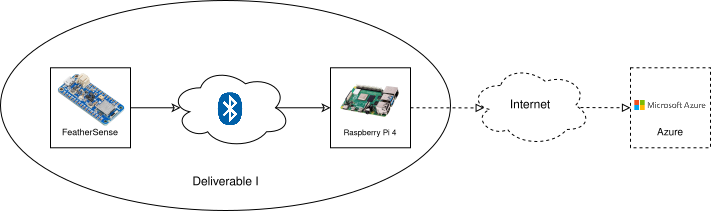
\includegraphics[width=0.5\textwidth]{media/basic_diagram.png}
	\caption{Block diagram of the IoT system, showing the layered design from sensing to future cloud integration.}
	\label{fig:block_diagram}
\end{figure}


\subsection{Simplified IoT architecture}

The system follows a simplified three-layer IoT architecture. The Sensing and Perception Layer is composed of a wearable sensor node, a compact hip-worn device with a 6-axis IMU for motion capture, where 3 axes are provided by the accelerometer and 3 axes are provided by the gyroscope, giving access to detailed movement information. The device also features a microcontroller with an accompanying BLE module, a battery management system module, and a rechargeable battery.

The Gateway / Edge Compute Layer features an IoT Gateway with a BLE module for collecting data from multiple sensor nodes, internet connectivity (by WiFi or Ethernet), and a powerful system-on-chip capable of data filtering, windowing, and feature extraction in real-time for multiple wearable devices. It is intended to be a stationary gateway mounted in a central location where it can capture data from many devices, process it, and push it to a cloud data processing pipeline.

The Application Layer consists of a machine-learning and data analytics pipeline where a machine learning model classifies the current activity using the received data. The classification, time, and received data are saved in a time-series database for long-term storage, allowing healthcare professionals to access historical activity data for their patients, and configure alerting for patients who are idle for too long or who may be over-active during their recovery.


\section{Component Selections}\label{CS}

\subsection{Sensor Node}\label{SN}
The Adafruit FeatherSense nRF52840\cite{b7} was provided as the designated sensor node. This board integrates multiple sensors (e.g., accelerometer/gyroscope, magnetometer, microphone, temperature, humidity, and pressure sensors) along with native BLE support. For this project, only the accelerometer and gyroscope were used, as these correspond directly with the HARTH dataset \cite{b5,b6} chosen for activity recognition. The other onboard sensors were not relevant to the project aims and were therefore excluded.

Although platforms like the Espressif ESP32 DecKitC are used widely in other IoT projects, offering Wi-Fi and BLE connectivity \cite{b8}, they typically require an external intertial measurement unit (IMU) if accelerometer or gyroscope sensing is needed. This comes with an increased cost, complexity and board count. The FeatherSense nRF52840 on the other hand comes with an integrated LSM6DS3 IMU, native BLE, and USB \& Batter charging support in one package. This makes it more suitable for the project's requirements for a self contained inertial sensor node.


\subsection{Gateway}\label{GW}
The Raspberry Pi 4 served as the IoT gateway. This device was issued for this project, and it has the sufficient computing capacity, integrated BLE support, and compatibility with Python's data acquisition and processing libraries. 
\textbf{[@Sean: again, if you want to add anything here. I think from the brief maybe we do need to do some comparison, like what I did inthe last paragraph]} 

\subsection{Communication}\label{COM}
BLE was the protocol used, as it is the only wireless option natively supported by the FeatherSense nRF52840 board. An initial implementation used BLE UART with CBOR encoding. However this was too slow. To meet the 50~Hz sampling target, the system was reimplemented using BLE GATT, transmitting fixed length packets of six floating point values. This achieved stable operation at the required frequency.

\subsection{Power}
For prototyping, the FeatherSense was powered via USB, which ensured stability and ease of development. The board supports battery operation, but this was not implemented for Deliverable I, which focused on demonstrating data acquisition and transmission. In a full deployment scenario, low-power optimisation and battery usage would become essential for continuous wearable operation.

\textbf{[@Sean: IDk I can look at the code and see if there is anything we can do to help with power consumption, just to say yeah in future we can do this. Not sure fully what to say on this point.]} 



\section{Prototype Design Plan}

\subsection{Subsystems}
The prototype will be structured into four main subsystems: 
\begin{itemize}
	\item \textbf{Sensing:} inertial data acquisition from the FeatherSense accelerometer and gyroscope. 
	\item \textbf{Communication:} wireless transmission via BLE, using GATT as the chosen protocol. 
	\item \textbf{Edge Processing:} real-time data handling and basic feature extraction on the Raspberry Pi 4. 
	\item \textbf{Visualisation:} plotting of data streams to confirm correct reception and interpretation. 
\end{itemize}
This breakdown will ensure that each component of the system can be developed and validated independently before integration. 

\subsection{Integration Plan}
The system will be developed incrementally. The sensor subsystem will first be validated by confirming raw inertial readings on the FeatherSense. Next, BLE transmission will be tested in isolation before final integration. Finally, the gateway will be configured to receive and interpret packets, after which end to end data flow from sensing to visualisation will be verified. 


\textbf{[@Sean: idk really, if you have any thoughts on the above two sections.]}

\subsection{Verification Plan}
Verification activities will be designed to ensure that the prototype meets Deliverable~I requirements. The main checks will include:
\begin{itemize}
	\item Confirming that BLE transmission achieves the target 50~Hz sampling rate. 
	\item Ensuring data packets are correctly structured and fully decoded at the gateway. 
	\item Validating that received sensor values fall within expected physical ranges (e.g., acceleration values near $\pm 9.8~\text{m/s}^2$ for gravity). 
	\item Measuring packet loss rates to assess communication reliability. 
\end{itemize}


\subsection{Verification Plan}
Verification activities will be designed to ensure that the prototype meets Deliverable~I requirements. The main checks will include:
\begin{itemize}
	\item Confirming that BLE transmission achieved the target 50~Hz sampling rate. 
	\item Ensuring data packets were correctly structured and fully decoded at the gateway. 
	\item Validating that received sensor values were within expected physical ranges (e.g., acceleration values near $\pm 9.8~\text{m/s}^2$ for gravity). 
\end{itemize}

\textbf{[@Sean: again, some more stuff here maybe on what we are doing with regards verification. Will need to test packet loss. This verification section is just chatgpt nonsense atm]}

\section{Implementation}
\subsection{Feathersense Node Setup}
The sensor node was implemented using the Adafruit FeatherSense nRF52840 board. The LSM6DS3 IMU was configured to sample at 50Hz, in line with the publicly available HARTH dataset. Sensor readings (acceleration in m/s\textsuperscript{2} and angular velocity in deg/s) were acquired in real time through the Adafruit CircuitPython libraries. 

\subsection{Communication Performance}
An initial implementation used the Nordic UART Service over BLE, with payloads encoded in CBOR format. This implementation was functional, but very inneficient. The structured CBOR packets were relatively large, so the transmission was slower and there was an increased coding and decoding overhead on both device and gateway. As a result, the effective sampling rate was limited to approximately 11~Hz, and partial reads often caused incomplete or dropped data. The performance was too poor to be considered as an option, and further measurements of latency or packet loss were not taken in this configuration. 

To address the issues found with the UART method, the system was reimplemented using a custom GATT service with two vendor-defined UUIDs (one for the service and one for the sensor characteristic). Instead of transmitting dictionary structures, the new approach packed six 32 bit floating point values (ax, ay, az, gx, gy, gz) into a fixed length 24 byte payload. This enabled stable streaming at the target rate of 50~Hz without the packet corruption or decoding delays observed previously.

\textbf{[TODO: Record and report packet loss statistics in current implementation.]} 




\section{Implementation of Gateway Device}
\textbf{[@Sean: I'll leave this to you]} 
\subsection{Data collection on Raspberry Pi}
connection with Feathersense via BLE GATT.

\subsection{Streaming Visualisation}
 live plotting of received sensor data.

(Screenshots/graphs of plots go here.)

\section{Edge/Fog Processing}
Jerk calculation (derivative of acceleration).

Magnitude of accel/gyro.

Other features relevant for ML (you can mention RMS, variance, etc. if planned).

Show small plots of raw vs processed features.


\subsection{Discussion \& Conclusion}
\textbf{[@Sean: this once we've done the rest of course]} 
Summary: successful acquisition, transmission, preprocessing.

Limitations: still simulated/early prototype, real-world testing needed.

Next steps (for Deliverable II): deploy ML in cloud, integrate with Power BI.

\bibliographystyle{IEEEtran}
\bibliography{references}


\end{document}